\documentclass[12pt]{article}
\usepackage[utf8]{inputenc}

\usepackage{lmodern}

\usepackage{enumitem}
\usepackage[margin=2cm]{geometry}

\usepackage{amsmath, amsfonts, amssymb}
\usepackage{graphicx}
%\usepackage{subfigure}
\usepackage{tikz}
\usepackage{pgfplots}
\usepackage{multicol}

\usepackage{comment}
\usepackage{url}
\usepackage{calc}
\usepackage{subcaption}
\usepackage[indent=0pt]{parskip}

\usepackage{array}
\usepackage{blkarray,booktabs, bigstrut}

\pgfplotsset{compat=1.16}

% MATH commands
\newcommand{\ga}{\left\langle}
\newcommand{\da}{\right\rangle}
\newcommand{\oa}{\left\lbrace}
\newcommand{\fa}{\right\rbrace}
\newcommand{\oc}{\left[}
\newcommand{\fc}{\right]}
\newcommand{\op}{\left(}
\newcommand{\fp}{\right)}

\newcommand{\bi}{\mathbf{i}}
\newcommand{\bj}{\mathbf{j}}
\newcommand{\bk}{\mathbf{k}}
\newcommand{\bF}{\mathbf{F}}

\newcommand{\mR}{\mathbb{R}}

\newcommand{\ra}{\rightarrow}
\newcommand{\Ra}{\Rightarrow}

\newcommand{\sech}{\mathrm{sech}\,}
\newcommand{\csch}{\mathrm{csch}\,}
\newcommand{\curl}{\mathrm{curl}\,}
\newcommand{\dive}{\mathrm{div}\,}

\newcommand{\ve}{\varepsilon}
\newcommand{\spc}{\vspace*{0.5cm}}

\DeclareMathOperator{\Ran}{Ran}
\DeclareMathOperator{\Dom}{Dom}

\newcommand{\exo}[3]{\noindent\textcolor{red}{\fbox{\textbf{Section {#1} | Problem {#2} | {#3} points}}}\\}
\newcommand{\qu}[2]{\noindent\textcolor{red}{\fbox{\textbf{Section {#1} | Problem {#2}}}}\\}

\begin{document}
	\noindent \hrulefill \\
	MATH-302 \hfill Pierre-Olivier Paris{\'e}\\
	Homework 9 Problems \hfill Fall 2022\\\vspace*{-1cm}
	
	\noindent\hrulefill
	
	\spc
	
	\exo{7.1}{A}{5}
	\\
	We have
		\begin{align*}
		(1 - x)^{-1} = \sum_{n = 0}^\infty x^n .
		\end{align*}
	We differentiate, we then get
		\begin{align*}
		\frac{d}{dx} \Big( \frac{1}{1 - x} \Big) = \sum_{n =1}^\infty n x^{n - 1}
		\end{align*}
	and this gives
		\begin{align*}
		-\frac{1}{(1 - x)^2} = \sum_{n = 1}^\infty n x^{n - 1} .
		\end{align*}
	
	\newpage
	
	\exo{7.1}{B}{20}
	\\
	Let $y (x) = \sum_{n = 0}^\infty a_n x^n$. We have
		\begin{align*}
		y' (x) = \sum_{n = 1}^\infty n a_n x^{n - 1} 
		\end{align*}
	and so the left-hand side becomes
		\begin{align*}
		& \sum_{n = 1}^\infty n a_n x^{n - 1} + x = \sum_{n = 1} n x^n \\
		\iff & a_1 + (2a_2 + 1) x + \sum_{n = 2}^\infty (n +1) a_{n + 1} x^n = x + \sum_{n = 2}^\infty n x^n .
		\end{align*}
	Comparing coefficients, we find
		\begin{align*}
		a_1 = 0 , \quad 2a_2 + 1 = 1 \quad \text{and} \quad (n + 1) a_{n + 1} = n \quad (n \geq 2)
		\end{align*}
	and therefore
		\begin{align*}
		a_1 = 0 , \quad a_2 = 0 \quad \text{and} \quad a_{n + 1} = \frac{n}{n + 1} \quad (n \geq 2) .
		\end{align*}
	The solution is therefore
		\begin{align*}
		y(x) = a_0 + \sum_{n = 2}^\infty \frac{n}{n + 1} x^n .
		\end{align*}
	
	We have $y (0) = 0$, then $a_0 = 0$. So, the solution is
		\begin{align*}
		y(x) = \sum_{n = 2}^\infty \frac{n}{n + 1} x^n .
		\end{align*}
		
	\underline{Remark:} We can find a close formula for the solution. We have
		\begin{align*}
		\sum_{n = 2}^\infty \frac{n}{n + 1} x^n = \sum_{n = 2}^\infty x^n - \sum_{n = 2}^\infty \frac{x^n}{n + 1} = \sum_{n = 0}^\infty x^n - 1 - x - \frac{1}{x} \sum_{n = 2}^\infty \frac{x^{n + 1}}{n + 1}
		\end{align*}
	and using the power series representation of $(1 - x)^2$ and $- \ln (1 - x)$, we then find that
		\begin{align*}
		y(x) &= \frac{1}{1 - x} - 1 - x + \frac{1}{x} \Big( x + \frac{x^2}{2} + \ln (1 - x) \Big) \\
		&= \frac{1}{1 - x} - \frac{x}{2} + \frac{1}{x} \log (1 - x) .
		\end{align*}
		
	\newpage
	
	\exo{7.1}{C}{5}
	\\
	Since the power series of $(1 - x)^{-1}$ is
		\begin{align*}
		\sum_{n = 0}^\infty x^n ,
		\end{align*}
	we have
		\begin{align*}
		T_N (x) = 1 + x + x^2 + \cdots + x^{N-1} + x^N .
		\end{align*}
	Below, we used Desmos to plot the graph of $T_4$, $T_10$, $T_{20}$. The graph of $(1 - x)^{-1}$ is in green.
	
	\begin{figure}[h]
	\centering
		\begin{subfigure}[b]{0.32\textwidth}
		\centering
		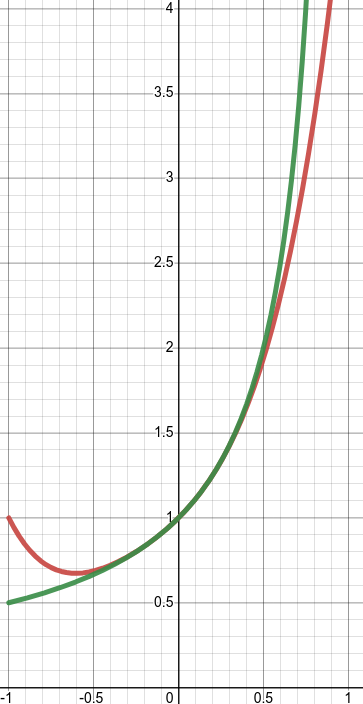
\includegraphics[scale=0.40]{fig1.png}
		\caption{$T_4$}
		\end{subfigure}
		\begin{subfigure}[b]{0.32\textwidth}
		\centering
		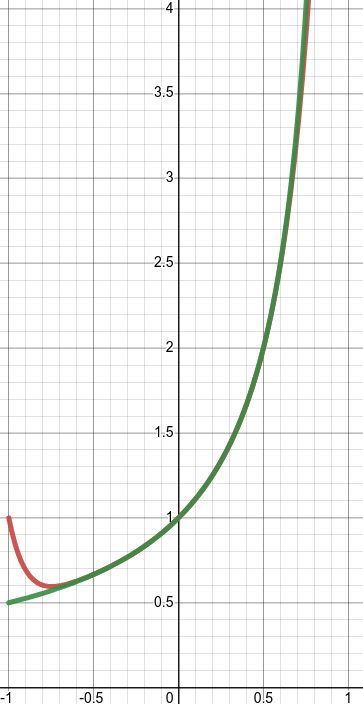
\includegraphics[scale=0.40]{fig2.png}
		\caption{$T_{10}$}
		\end{subfigure}
		\begin{subfigure}[b]{0.32\textwidth}
		\centering
		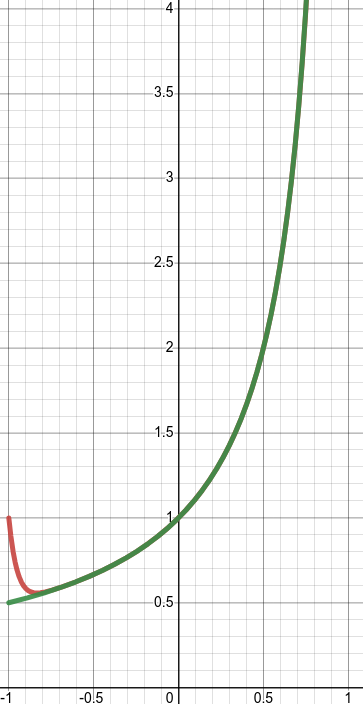
\includegraphics[scale=0.40]{fig3.png}
		\caption{$T_{20}$}
		\end{subfigure}
	\end{figure}
	
	\newpage
	
	\exo{7.1}{D}{10}
	\\
	Set $y(x) = \sum_{n = 0}^\infty a_n x^n$. We have
		\begin{align*}
		y' (x) = \sum_{n =1}^\infty n a_n x^{n - 1} \quad \text{ and } \quad y'' (x) = \sum_{n = 2}^\infty n (n - 1) a_nx^{n - 2} .
		\end{align*}
	Therefore, we get
		\begin{align*}
		x^2 y'' &= \sum_{n = 2}^\infty n (n - 1) a_n x^n \\
		2x y' &= \sum_{n = 1}^\infty 2 n a_n x^n \\
		3x y &= \sum_{n = 0}^\infty 3 a_n x^{n + 1} .
		\end{align*}
	We then get
		\begin{align*}
		x^2 y'' + 2x y' - 3xy &= \sum_{n = 2}^\infty n (n - 1) a_n x^n + \sum_{n = 1}^\infty 2 n a_n x^n - \sum_{n = 0}^\infty 3 a_n x^{n + 1} \\
		&=  \sum_{n = 2}^\infty n (n - 1) a_n x^n + \sum_{n = 1}^\infty 2 n a_n x^n - \sum_{n = 1}^\infty 3 a_{n-1} x^{n} \\
		&= (2a_1 - 3a_0) x + \sum_{n= 2}^\infty \Big( \big( n(n-1) + 2n \big) a_n - 2 a_{n-1} \Big) x^n \\
		&= (2a_1 - 3a_0)x + \sum_{n = 2}^\infty \Big( n (n + 1) a_n - 2a_{n-1} \Big) x^n .
		\end{align*}
	Therefore, the expression can be rewritten as a power series $\sum_{n = 0}^\infty c_n x^n$, where
		\begin{align*}
		c_0 = 0 , \quad c_1 = 2a_1 - 3a_0 \quad \text{ and } \quad c_n = n (n + 1) a_n - 2 a_{n-1} .
		\end{align*}
		
	\newpage
	
	\exo{7.1}{E}{10}
	\\
	Let $y (x) = \sum_{n = 0}^\infty a_n x^n$. Then, we have
		\begin{align*}
		y' (x) = \sum_{n =1}^\infty n a_n x^{n - 1} \quad \text{ and } \quad y'' (x) = \sum_{n = 2}^\infty n (n - 1) a_nx^{n - 2} .
		\end{align*}
	We therefore get
		\begin{align*}
		x y'' &= \sum_{n = 2}^\infty n (n- 1)a_n x^{n-1} \\
		(4 + 2x) y' &= \sum_{n = 0}^\infty 4a_n x^n + \sum_{n = 1}^\infty 2n a_n x^n \\
		(2 + x) y &= \sum_{n = 0}^\infty 2a_n x^n + \sum_{n = 0}^\infty a_n x^{n + 1} .
		\end{align*}
	We can therefore get
		\begin{align*}
		xy'' + (4 + 2x) y' + (2 + x) y &= \sum_{n = 2}^\infty n (n- 1)a_n x^{n-1}  + \sum_{n = 0}^\infty 4a_n x^n + \sum_{n = 1}^\infty 2n a_n x^n + \sum_{n = 0}^\infty 2a_n x^n + \sum_{n = 0}^\infty a_n x^{n + 1} \\
		&= \sum_{n = 1}^\infty (n + 1)n a_n x^n + \sum_{n = 0}^{\infty} (6 + 2n) a_n x^n + \sum_{n = 1}^\infty a_{n-1} x^n \\
		&= 6a_0 + \sum_{n = 1}^\infty \Big( (n^2 + n + 2n + 6) a_n + a_{n-1} \Big) x^n \\
		&= 6a_0 + \sum_{n = 1}^\infty \Big( (n^2 + 3n + 6) a_n + a_{n-1} \Big) x^n .
		\end{align*}
	We can then rewrite the expression as a power series $\sum_{n =0}^\infty c_n x^n$ with
		\begin{align*}
		c_0 = 6a_0 \quad \text{and} \quad c_n = (n^2 + 3n + 6) a_n + a_{n - 1} .
		\end{align*}
	
	\vfill
	
	\hfill \textcolor{red}{\textsc{Total (Points): 50.}}
	
	
	
\end{document}